\chapter{Einleitung}

\section{Motivation}

Bei den Themenbereichen Big Data und Data Mining handelt es sich um Teilgebiete der Informatik, die in den vergangenen Jahren stark an Bedeutung gewonnen haben und daher aktuell von hohem Interesse sind. Es geht dabei um die Beschaffung, Analyse und Interpretation großer Datenmengen zur Gewinnung zusätzlicher Informationen. Aufgrund der Bedeutung und Aktualität dieser Gebiete war dementsprechend auch die Motivation der Projektteilnehmer groß, aktiv in diesem Bereich zu arbeiten und teilweise bereits vorhandene theoretische Kenntnisse in die Praxis umzusetzen. Ein ebenso bedeutsames Anwendungsgebiet dafür sind soziale Netzwerke, welche zudem den Vorteil besitzen, große Datenmengen öffentlich zur Verfügung zu stellen. Unsere Wahl fiel daher auf den Kurznachrichtendienst Twitter.

Damit war eine sehr allgemeine Projektidee unter der Überschrift "`Data Mining auf Twitter"' gefunden. Um jedoch ein tatsächliches Projekt in der zur Verfügung stehenden Zeit umsetzen zu können, musste diese Idee auf einen spezifischen Anwendungsbereich konkretisiert werden. Vor dem offiziellen Beginn des Projekts bestanden dazu bereits von unterschiedlichen Projektmitgliedern eingebrachte Vorschläge. Diese basierten einerseits auf der Erkenntnis, dass sich die Aktivität auf Twitter möglicherweise mit der Bedeutung oder Aktualität eines bestimmten Themas in Verbindung setzen lässt, während der Inhalt der geposteten Nachrichten (auch Tweets genannt) einen Rückschluss auf die allgemeine Stimmung zu einem diskutierten Thema zulässt. Dieser Zugang erschien uns sinnvoll, da es interessant ist, ob sich aus den vorhandenen Informationen ein aussagekräftiges und realistisches Meinungsbild gewinnen lässt. Außerdem erfordert eine solche Analyse den Einsatz von Verfahren aus dem \textit{Machine Learning}, ein weiteres aktuelles Gebiet, in dem sich wertvolle Erfahrungen sammeln lassen. Auf der anderen Seite ließ sich aus unserer Sicht die Tatsache nutzen, dass Tweets eine räumliche und zeitliche Dimension aufweisen, das heißt es ist bekannt, wo und wann ein Tweet erstellt wurde. Das eröffnet die Möglichkeit, die Popularität eines Themas zeitlich nachzuvollziehen oder seine räumliche Ausbreitung darzustellen. Abhängig von der Komplexität dieser räumlichen Analyse ließen sich hier auch Verfahren aus der algorithmischen Geometrie einbringen. Als eine anfängliche praktische Anwendung dieser Betrachtungsweisen wurde zunächst die Politik vorgeschlagen. Das stand unter dem Eindruck gesellschaftlicher Entwicklungen, in denen Twitter eine Rolle spielte, wie z.\,B. des arabischen Frühlings und ähnlicher Protestbewegungen. Die Verbreitungen solcher Entwicklungen lassen sich beispielsweise räumlich nachvollziehen. Als Anwendung des Meinungsbildes war vorgesehen, eine Aussage über den Ausgang von Wahlen treffen zu können.

Für die Organisation der Umsetzung dieser Ideen wurden Verfahren der agilen Software-Entwicklung eingesetzt. 
Dies sollte den Projektmitgliedern ermöglichen, Erfahrungen mit den damit verbundenen Vorgehensweisen und Prinzipien wie beispielsweise Scrum zu sammeln und dem Projekt zusätzlich zum akademischen auch einen praktischen Charakter verleihen. 
Das ist besonders unter dem Hinblick von Bedeutung, dass sich die Anforderungen im Projektverlauf ständig verändern können und das Team in der Lage sein muss, darauf zu reagieren.
%Auf diese Weise konnten die Projektmitglieder Erfahrungen mit den damit verbundenen Vorgehensweisen und Prinzipien wie beispielsweise Scrum sammeln und das Projekt als Ganzes erhielt einen eher praxisnahen und weniger akademischen Charakter. 
%Da die Produktbetreuer jeweils die Rollen des Product Owner und des Kunden einnahmen und wöchentlich Kundengespräche mit neuen Anforderungen aus der Perspektive eines naiven Benutzers stattfanden, ermöglichte diese Vorgehensweise auch eine kontinuierliche Weiterentwicklung der Idee im Verlauf des Projekts. Das wichtigste Konzept, das aus diesen Rückmeldungen hervorging, war dabei das Prinzip des explorativen Arbeitens. Damit ist gemeint, dass der Benutzer bei jeder bereitgestellten Analyse die Möglichkeit haben soll, die Grundlage dieser Ergebnisse herausfinden zu können.

\section{Umgesetztes System}
\label{sec:umgesetztesSystem}

Aus diesem Prozess ging schlussendlich der finale Zustand des Systems hervor. Wie bereits erläutert, war die Grundidee, zu einem spezifischen Thema oder Begriff die Daten aus Twitter aus einer Reihe verschiedener Gesichtspunkte darzustellen. Das System sollte dabei als Anwendung im Browser realisiert werden, wobei wir uns im Hinblick auf Eleganz und Bedienbarkeit an Seiten wie Wolfram Alpha\footnote{\url{www.wolframalpha.com}} orientiert haben. Aus diesem Grund besteht die Startseite der Anwendung nur aus einem Eingabefeld für den gewünschten Suchbegriff.

Ist ein Suchbegriff eingegeben, beginnt die Analyse. Dabei wird unterschieden, ob in unserer Datenbank bereits Daten für diesen Begriff vorliegen oder nicht. Falls noch keine Daten vorhanden sind, wird der Suchbegriff in die Datenbank eingetragen und es wird damit begonnen, Daten zu diesem Suchbegriff von Twitter abzurufen und abzuspeichern. Wenn dann Daten vorhanden sind, werden die Daten von unserem System analysiert und anschließend dem Benutzer angezeigt. Wie bereits erwähnt, liegen die Ergebnisse nach spezifischen Gesichtspunkten vor, welche jeweils in Boxen dargestellt werden, die wir als Ansichten bezeichnen. Als Reaktion auf die Rückmeldung, dass die Menge der so präsentierten Informationen überwältigend oder ablenkend sein kann, wenn man nur an bestimmten Ergebnissen interessiert ist, wurde von uns die Option eingebaut, bestimmte Ansichten ein- oder auszublenden.

\begin{figure}[h!]
\centering
\begin{subfigure}[t]{0.45\textwidth}
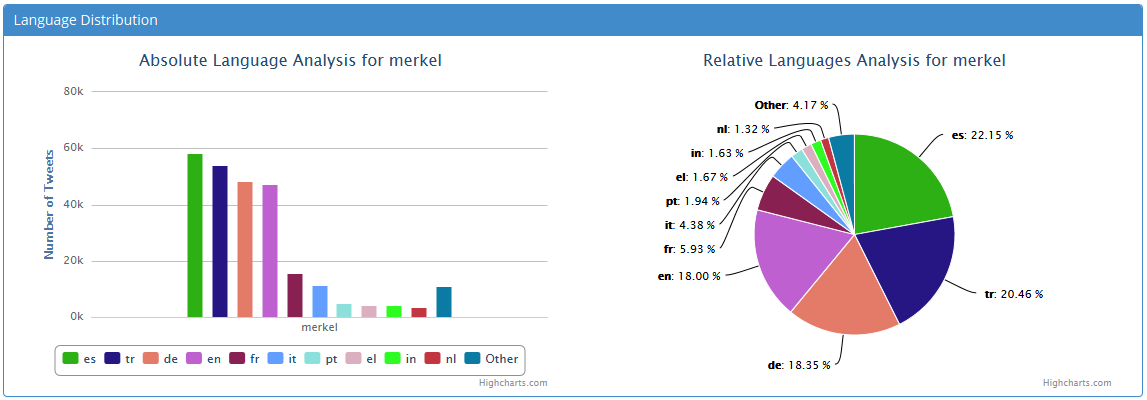
\includegraphics[width=\textwidth]{Bilder/Frontend/Screenshots/latestLanguageDistributionMerkel.png}
\caption{Sprachverteilung zu \glqq Merkel\grqq}
\label{fig:viewLanguageDistirbution}
\end{subfigure}
~
\begin{subfigure}[t]{0.45\textwidth}
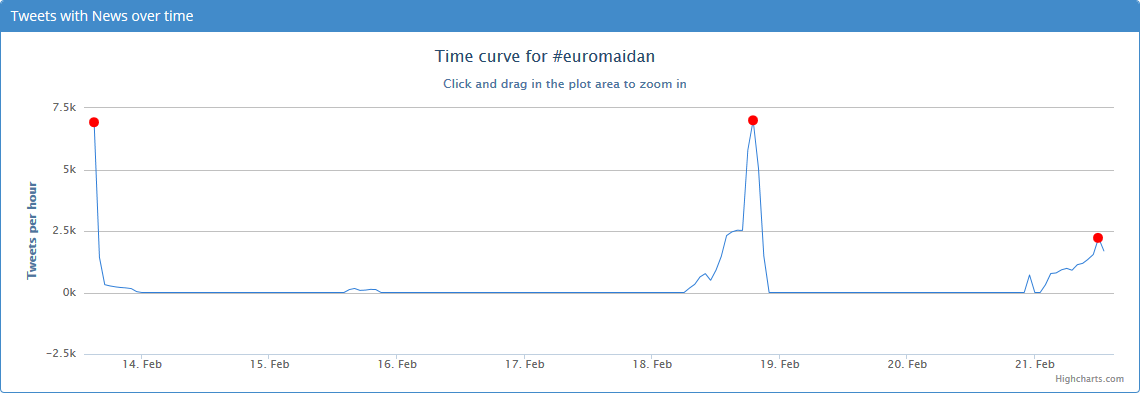
\includegraphics[width=\textwidth]{Bilder/Frontend/Screenshots/latestTweetsPerHourEuromaidan.png}
\caption{Anzahl Tweets im zeitlichen Verlauf zu \glqq \#euromaidan\grqq}
\label{fig:viewTweetsPerHour}
\end{subfigure}

\begin{subfigure}[t]{0.45\textwidth}
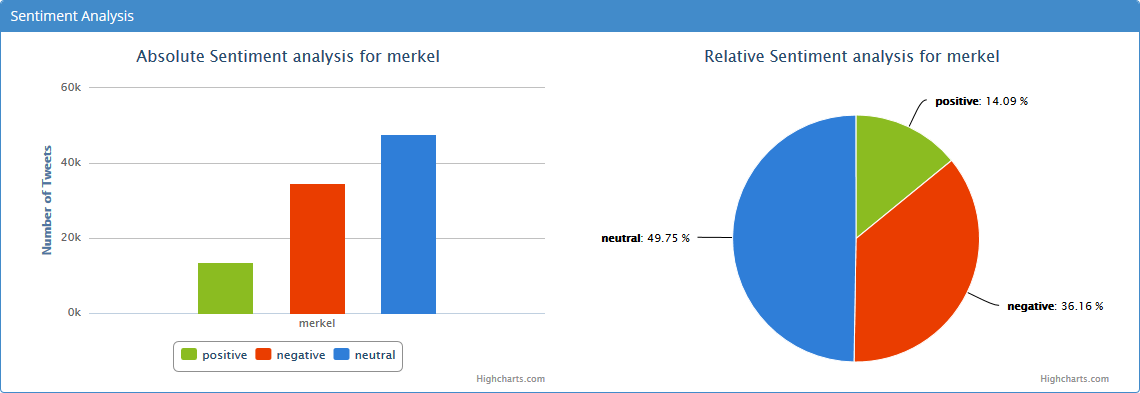
\includegraphics[width=\textwidth]{Bilder/Frontend/Screenshots/latestSentimentAnalysisMerkel.png}
\caption{Sentimentanalyse zu \glqq Merkel\grqq}
\label{fig:viewSentimentAnalysis}
\end{subfigure}
~
\begin{subfigure}[t]{0.45\textwidth}
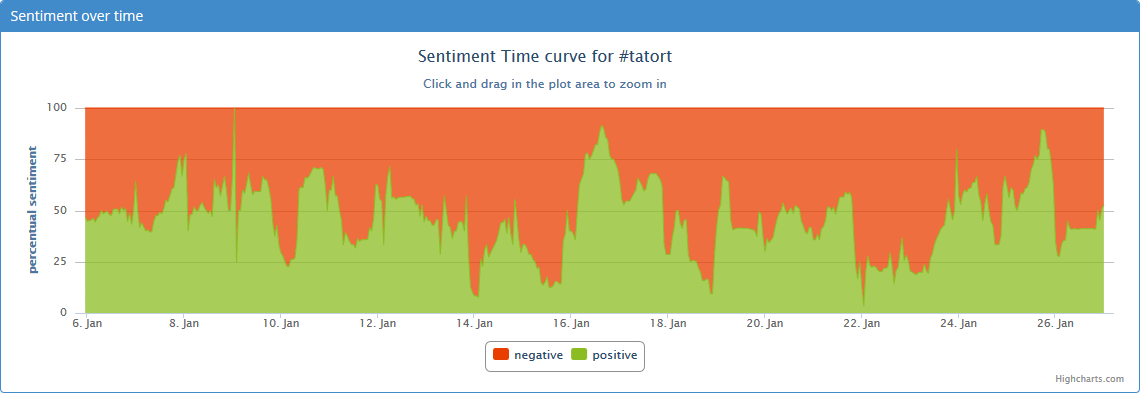
\includegraphics[width=\textwidth]{Bilder/Frontend/Screenshots/latestSentimentPerHourTatort.png}
\caption{Relatives Sentiment im zeitlichen Verlauf zu \glqq \#tatort\grqq}
\label{fig:viewSentimentPerHour}
\end{subfigure}

\begin{subfigure}[t]{0.45\textwidth}
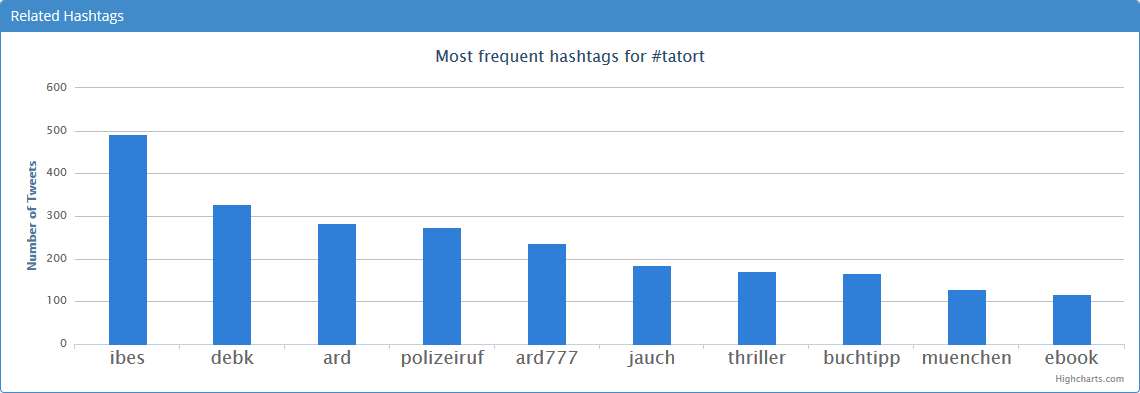
\includegraphics[width=\textwidth]{Bilder/Frontend/Screenshots/latestRelatedHashtagsTatort.png}
\caption{Verwandte Hashtags zu \glqq \#tatort\grqq}
\label{fig:viewRelatedHashtags}
\end{subfigure}
~
\begin{subfigure}[t]{0.45\textwidth}
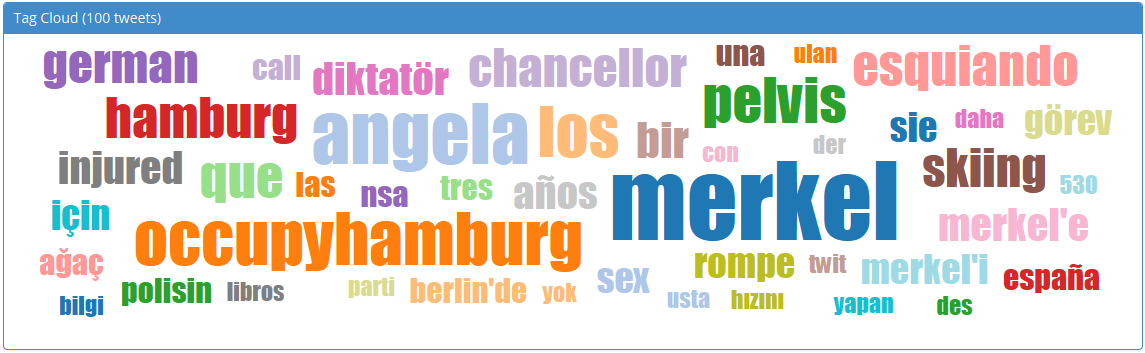
\includegraphics[width=\textwidth]{Bilder/Frontend/Screenshots/latestTagCloudMerkel.png}
\caption{Tag Cloud zu \glqq Merkel\grqq}
\label{fig:viewTagCloud}
\end{subfigure}

\begin{subfigure}[t]{0.45\textwidth}
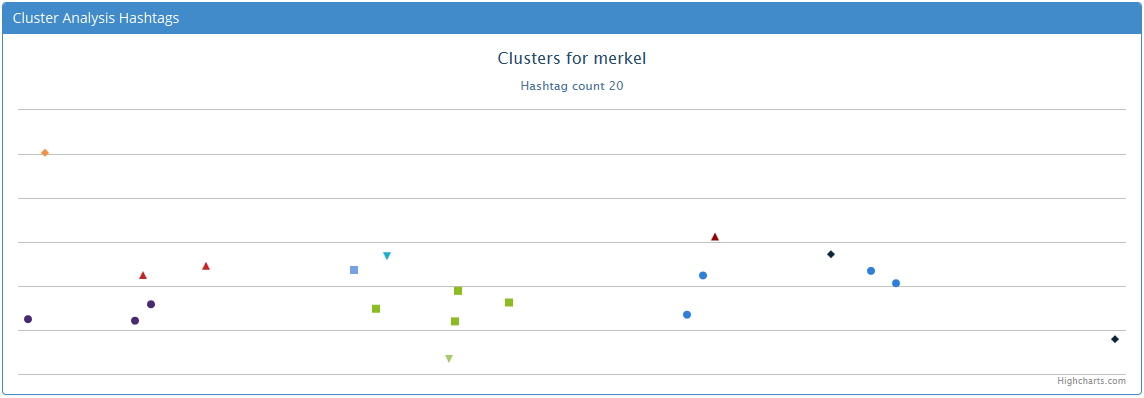
\includegraphics[width=\textwidth]{Bilder/Frontend/Screenshots/latestClusterHashtagMerkel.png}
\caption{Cluster-Analyse von Hashtags zu \glqq Merkel\grqq}
\label{fig:viewClusterHashtags}
\end{subfigure}
~
\begin{subfigure}[t]{0.45\textwidth}
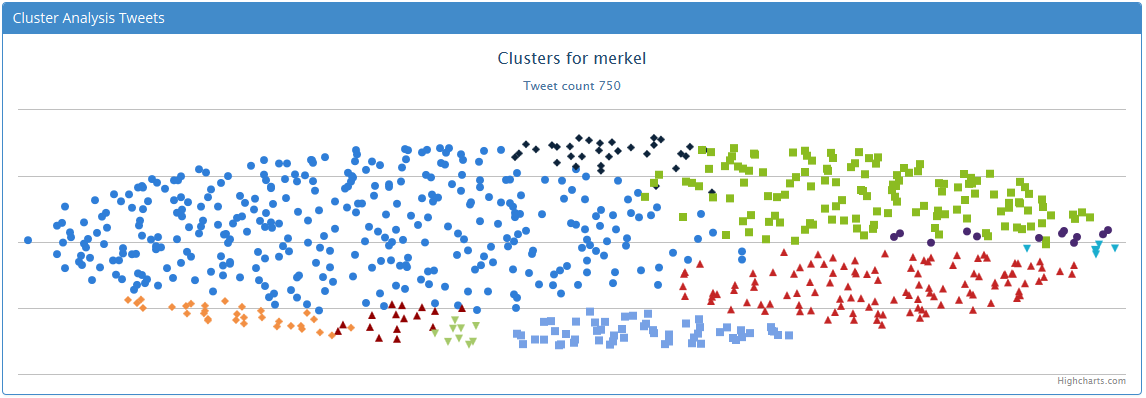
\includegraphics[width=\textwidth]{Bilder/Frontend/Screenshots/latestClusterTweetsMerkel.png}
\caption{Cluster-Analyse von Tweets zu \glqq Merkel\grqq}
\label{fig:viewClusterTweets}
\end{subfigure}
\caption{Alle acht Ansichten unseres Systems}
\label{fig:viewScreenshots}
\end{figure}

In der finalen Version unseres Systems sind acht verschiedene Ansichten enthalten, die in Abbildung \ref{fig:viewScreenshots} zu sehen sind. Fünf dieser Ansichten sind Umsetzungen der im vorigen Abschnitt beschriebenen, ursprünglichen Projektidee. Die drei weiteren Ansichten entstanden im Verlauf des Projektes auf Wunsch des Kunden, einen besseren Überblick über diesen Suchbegriff zu erhalten.
Das Stimmungsbild zu einem Thema wird in der \glqq Sentimentanalyse\grqq{} (\ref{fig:viewSentimentAnalysis}) betrachtet, bei der jedem Tweet eine positive, negative oder neutrale Stimmung (Sentiment) zugewiesen ist. Die zeitliche Ausbreitung ist in der Ansicht \glqq Tweets im zeitlichen Verlauf"' (\ref{fig:viewTweetsPerHour}) zu sehen, welche die Anzahl Tweets zum Suchbegriff pro Stunde auf einem Graphen aufträgt. Eine Kombination aus Stimmungsbild und zeitlicher Ausbreitung wird in der Ansicht \glqq Relatives Sentiment im zeitlichen Verlauf\grqq{} (\ref{fig:viewSentimentPerHour}) angeboten.
Das Clustering von Tweets gemäß ihrer Gemeinsamkeiten ist in der Ansicht \glqq Cluster-Analyse von Tweets\grqq{} (\ref{fig:viewClusterTweets}) umgesetzt worden. Eine Variation dieses Ansatzes findet sich in der \glqq Cluster-Analyse von Hashtags\grqq{} (\ref{fig:viewClusterHashtags}), bei der -- wie der Name schon vermuten lässt -- an Stelle von einzelnen Tweets Hashtags zu einem Suchbegriff zu Clustern zusammengefasst werden.
Die dort auftauchenden Hashtags sind allesamt Tweets zu diesem Suchbegriff entnommen. Eine Übersicht über die häufigsten dieser Hashtags bietet die Ansicht \glqq Verwandte Hashtags\grqq{} (\ref{fig:viewRelatedHashtags}), welche die zehn meistbenutzten Hashtags zum eingegeben Suchbegriff auflistet. Eine Verallgemeinerung dieser Ansicht ist die \glqq Tag Cloud\grqq{} (\ref{fig:viewTagCloud}), in der nicht nur Hashtags, sondern generell alle Worte (bis auf Worte ohne eigentlichen Informationsgehalt, sogenannte \textit{stop words}) ihrer Häufigkeit entsprechend angezeigt werden. Dabei wird die Häufigkeit eines Wortes durch die Größe der Darstellung repräsentiert: Je größer ein Wort dargestellt wird, desto häufiger ist es in Tweets zum analysierten Suchbegriff vorhanden. Außerdem existiert noch die \glqq Sprachverteilung\grqq{} (\ref{fig:viewLanguageDistirbution}), welche die absolute und relative Häufigkeit der Sprachen, in denen die Tweets eines Suchbegriffs verfasst sind, grafisch präsentiert.

Die Ergebnisse zu einem Suchbegriff werden in der Anzeige in einem Tab zusammengefasst, in dem die einzelnen Ansichten angezeigt werden. Bei der Suche nach weiteren Begriffen wird jeweils ein weiterer Tab hinzugefügt, der wiederum die einzelnen Ansichten enthält. Bei der Analyse von zwei oder mehr Suchbegriffen wird zudem ein weiterer Tab mit einer Vergleichsansicht aller eingegebenen Suchbegriffe präsentiert. Diese Vergleichsansicht enthält eine Ansicht zum Vergleich der Stimmungsbilder und eine Ansicht zum Vergleich der zeitlichen Verläufe der einzelnen Suchbegriffe, was in Abbildung \ref{fig:compare} zu sehen ist.

\begin{figure}[h!]
\centering
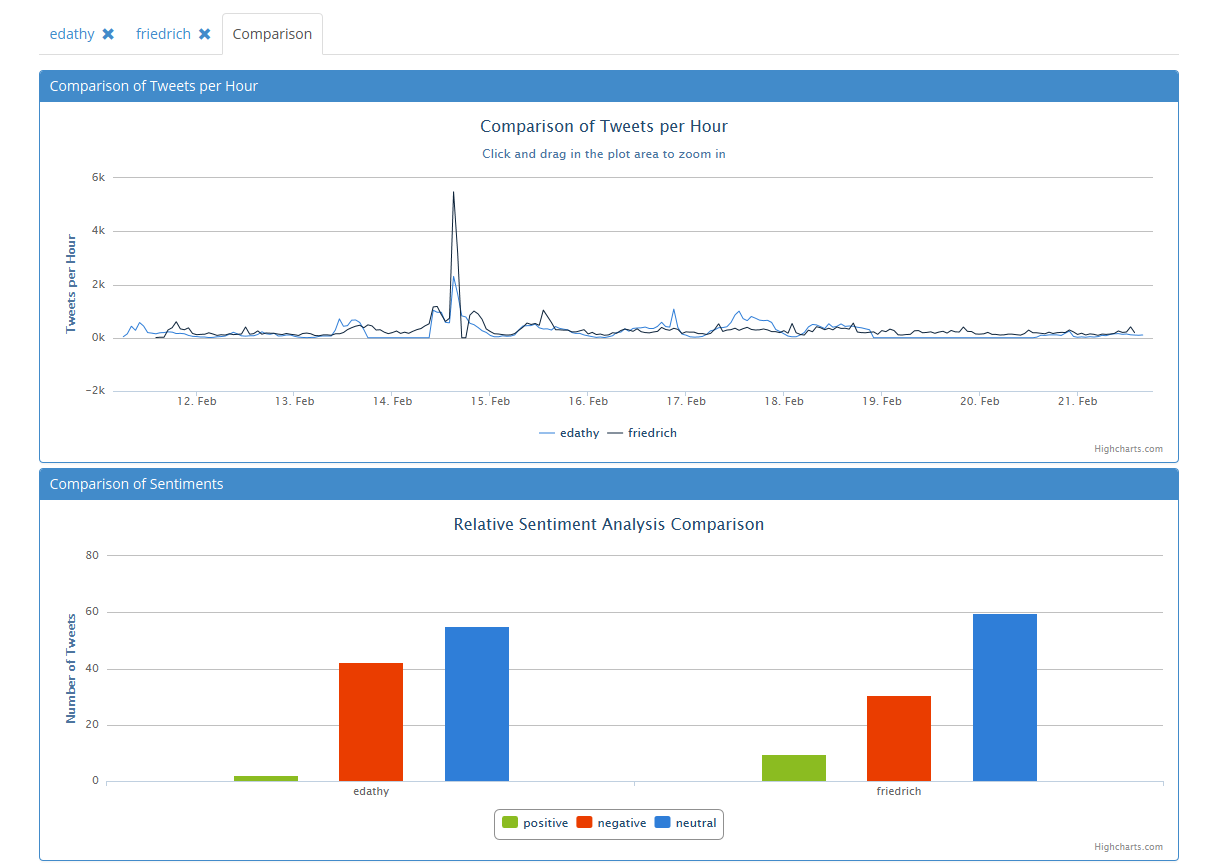
\includegraphics[width=0.8\textwidth]{Bilder/Frontend/Screenshots/comparison.png}
\caption{Vergleichsansicht zu den Suchbegriffen \glqq edathy\grqq{} und \glqq friedrich\grqq}
\label{fig:compare}
\end{figure}

Zusätzlich zur reinen Präsentation der analysierten Ergebnisse haben viele der soeben beschriebenen Ansichten auch Funktionalitäten, die exploratives Arbeiten mit dem System und den darin enthaltenen Daten ermöglicht. Beispielsweise ist es möglich, die zu analysierenden Daten zu einem Suchbegriff nach Sprachen zu filtern. Zusätzlich zum Sprachfilter in der Navigationsleiste ist diese Funktionalität auch aus der Ansicht \glqq Sprachverteilung\grqq\ verfügbar. Ebenso lässt sich die Suche nach einem weiteren Begriff nicht nur durch dessen Eingabe in die Suchleiste starten, sondern auch durch einen Klick auf den gewünschten Suchbegriff in der \glqq Tag Cloud\grqq\ oder bei \glqq verwandten Hashtags\grqq{}.
Eine Möglichkeit, detaillierte Informationen zu erhalten, bietet die Anzeige einzelner Tweets in unserem System. In der Ansicht zur \glqq Cluster-Analyse von Tweets\grqq\ ist dies durch einen Tooltip realisiert, in den Ansichten \glqq Sentimentanalyse\grqq\ und \glqq Tweets im zeitlichen Verlauf\grqq\ öffnet sich ein modaler Dialog mit einer detaillierten Anzeige von einzelnen Tweets.

Zusätzlich zur Anzeige einzelner Tweets bietet die Ansicht \glqq Tweets im zeitlichen Verlauf\grqq\ noch die Anzeige von News zu diesem Suchbegriff. Diese werden aus einer zusätzlichen Suche der drei externen Quellen \glqq Bing Web\grqq, \glqq Bing News\grqq\ und \glqq Google News\grqq\ akquiriert.
Dieses News-Modul wurde während des agilen Entwicklungsprozesses an Stelle des Kinomoduls umgesetzt, da eine Einbindung in das bis dahin bestehende System sowohl vom Product Owner, als auch von uns als sinnvoller erachtet wurde.
Eine weitere der ursprünglichen Projektideen, die aufgrund der Priorisierung durch den Product Owner herausfiel, ist die Anzeige der räumlichen Verbreitung von Tweets. Der Hauptgrund hierfür ist die relativ geringe Anzahl an Tweets, zu denen eine Position vorhanden ist.

In den folgenden Kapiteln wird das hier kurz beschriebene System und dessen Entstehungsprozess im Detail erläutert. Dazu wird in Kapitel \ref{cha:orga} zunächst beschrieben, wie wir das Projekt intern organisiert haben. Dies betrifft sowohl die Organisation des Systems als auch die von uns verwendete Vorgehensweise. Im darauf folgenden Kapitel \ref{cha:architektur} wird die Architektur unseres Systems beschrieben, welches in die drei grobe Bereiche Beschaffung, Analyse und Darstellung von Daten aufgegliedert ist. Die daraus entstandene Infrastruktur wird in Kapitel \ref{cha:infrastruktur} detailliert geschildert, woraufhin in Kapitel \ref{cha:komponenten} Details zu den einzelnen Komponenten und Ansichten gegeben werden. Das abschließende Kapitel \ref{cha:ausblick} fasst das zuvor Beschriebene kurz zusammen und bietet einen Ausblick auf mögliche weiterführende Ansätze, die auf dem von uns entwickelten System aufbauen.
